\chapter{Runway design}

	\section{Declared distances}
		\subsection{Runway 1}
	
		The first declared distance that will be calculated is the landing distance. Using the maximum landing weight (251.000kg) which can be found in the same paper and considering standard atmosphere conditions and sea level, the value can be obtained using the graph shown below: 
		
		\begin{figure}[H]
			\centering
			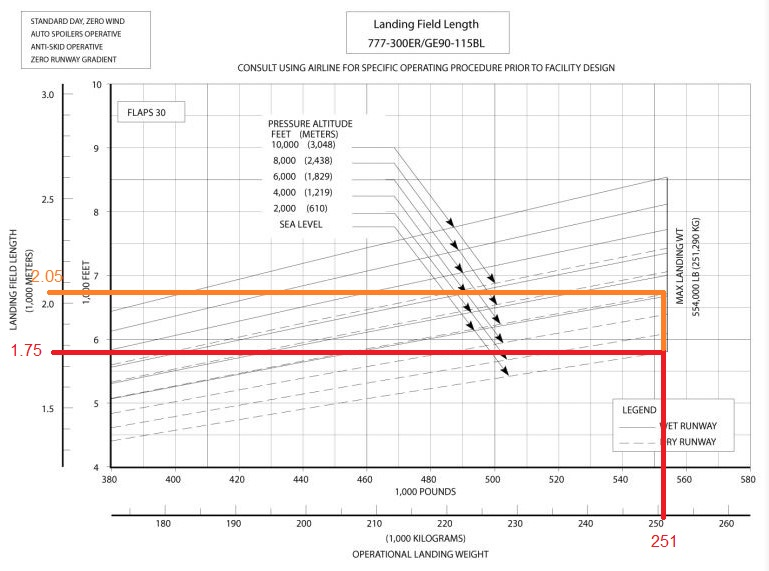
\includegraphics[clip, trim=0cm 0cm 0cm 0cm, width=1\textwidth]{./images/B777/landingdistance777}
			\label{} %per denotar una referencia
		\end{figure}
		
		The landing distance is 1.750m for dry runway and 2.050 for wet runway. Since the runway length is higher than those values, the available landing distance will be equal to the runway length.	Now, increasing its value by a coefficient of 67\%, the final landing distance obtained is 2.920m in dry runways and 3.417m. 
		
		The next distance that will be calculated is the takeoff length without engine failure (TODA). In order to calculate it, the reference field length (3.290m) will be corrected with a factor of 15\%.  The final TODA obtained is 3.783m.
		
		
		Moving into the takeoff length with engine failure (TORA), some hypotheses need to be done in order to calculate the final distance.  Due to the fact that the engine failure occurs after the critical velocity (v1) which is achieved at the 70\% of the runway total length, the thrust coefficient is reduced after that point. The final TORA obtained has a value of 4.120m.
		
		
		Finally, the last declared distance is the Accelerate-Stop Distance Available (ASDA). This distance also requires a hypothesis in order to be solved. The takeoff is cancelled before the critical velocity (v1), thus at the 65\% of the runway length. To compute the final ASDA, the landing distance has to be added to the 65\% of the runway length. The value obtained is 3890m.  
		
		All the declared distances obtained are minimum values, thus, in order to give them a safety margin, all the distances have been further increased. 
		
		\subsection{Runway 2}
	